\chapter{Performance analysis}

\label{Chapter4} 


In order to see which of the web technologies scores best, a performance benchmark was created. 
This benchmark uses Cypress to run a Lighthouse report for each PoC application.

The steps for running it are as follows:

\begin{enumerate}
	\item Start the CMS containers.
	      \begin{verbatim}
			docker-compose -f docker-compose-deps.yml up -d
	      \end{verbatim}
	      This will start a Postgres database and Strapi, the CMS. These must be ran before the others since the build scripts for the web applications require Strapi.
	\item Build all the PoC applications
	      	      	      	      	      	      	      	      	      	      	      	      	      	      	      	      	      	      	      	      	      	
	      \begin{verbatim}
			docker-compose -f docker-compose-bench.yml up -d
	      \end{verbatim}
	      This will build the applications and start the containers. 
	      You can access each application in the browser, starting with port 3000. (http://localhost:3000, http://localhost:3001, \dots)
	      	      	      	      	      	      	      	      	      	      	      	      	      	      	      	      	      	      	      	      	      
	\item  
	      	      	      	      	      	      	      	      	      	      	      	      	      	      	      	      	      	      	      
	      \begin{verbatim}
			cd packages/benchmark
			npm ci
			npm run cypress:open
	      \end{verbatim}
	      	      	      	      	      	      	      	      	      	      	      	      	      	      	      	      	      	      	      
	      This will install Cypress and its dependencies. 
	      After running the final command, Cypress will open and you are able to run the benchmark.
	      Reports with raw data will be saved in the packages/benchmark/reports directory.
\end{enumerate}

These are the steps to run the benchmark once. In order to get a statistically relevant measurement, a script in available that will run the benchmark multiple times.
At the top of the script, you'll find a variable TOTAL\_RUNS which you can adjust and will control how many times the benchmark is ran.
It can be run with

\begin{verbatim}
		cd packages/benchmark
		node runBenchmark.js
\end{verbatim}

Results from these benchmarking runs can be found in the file packages/benchmark/finalReport.json

Finally, you will find a Jupyter notebook that does some number crunching and renders the plots at packages/data-analysis/analysis.ipynb

Results with raw data can be found in appendix \ref{appendix:lighthouse-report}

\section{Largest contentful paint}

\begin{figure}[htb!]
	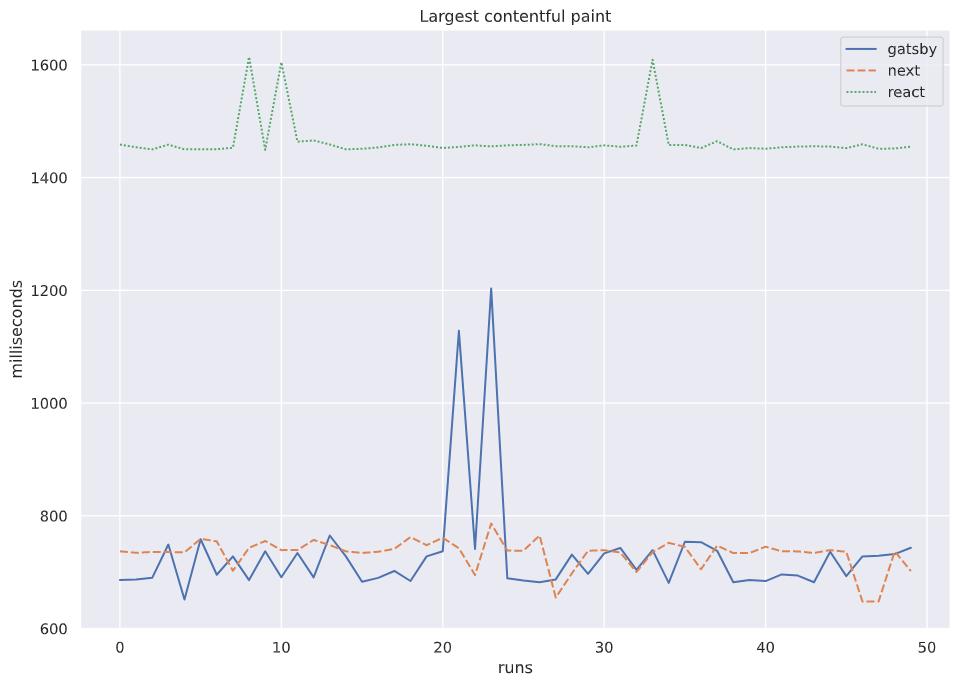
\includegraphics[scale=0.4]{largest_contentful_paint}{}
	\caption{Results of performance benchmark for largest contentful paint}
	\label{fig:largest_contentful_paint}
\end{figure}

In figure \ref{fig:largest_contentful_paint}, it is clear that LCP for a traditional React application is far greater than that of static site generators.

This makes sense: a traditional React application will perform many computational steps during runtime to render the DOM.
Static site generators will perform these computations during the build step.

\section{Total blocking time}


\begin{figure}[htb!]
	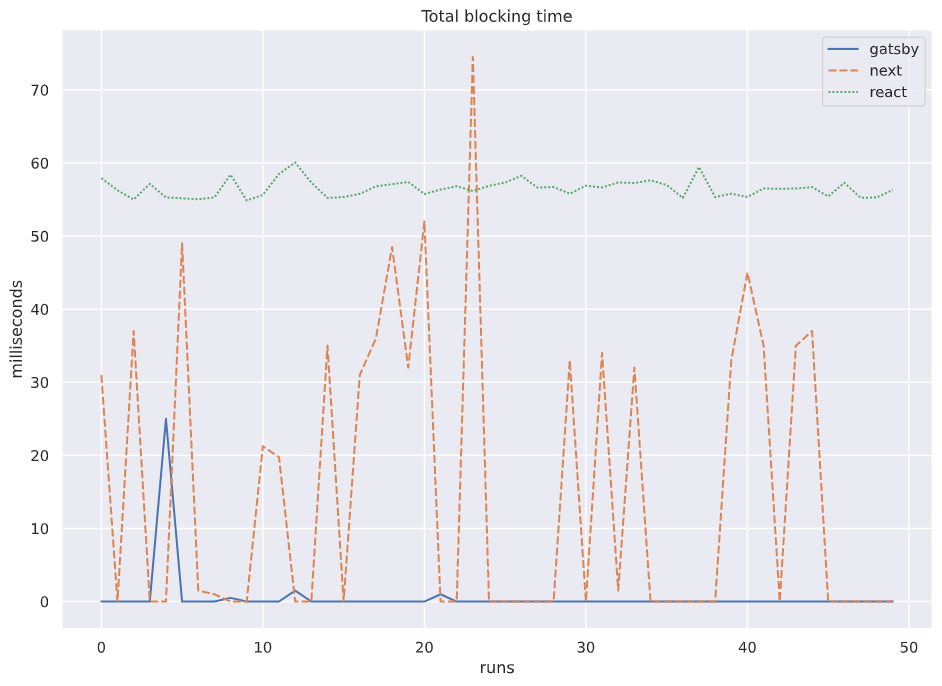
\includegraphics[scale=0.4]{total_blocking_time}
	\caption{Results of performance benchmark for total blocking time}
	\label{fig:total_blocking_time}
\end{figure}

In figure \ref{fig:total_blocking_time}, similar results to the previous figure can be observed
The traditional React application scores much less favorably than the static site generators.
Interestingly, the results for Next seem to spike a lot.

\section{Bundle size}

To measure the size of the resulting files after a production build was measured with the Unix command 

\begin{verbatim}
	du -c <directory>
\end{verbatim}

\begin{table}[htb!]
	\begin{center}
		\begin{tabular}{||c c||} 
			\hline
			Site   & Size \\ [0.5ex] 
			\hline\hline
			Gatsby & 3072 \\ 
			\hline
			Next   & 7012 \\
			\hline
			React  & 568  \\[1ex] 
			\hline
		\end{tabular}
		\caption{Total file size of production builds, in kilobytes }
		\label{tbl:bundle_size}
	\end{center}
\end{table}

Looking at table \ref{tbl:bundle_size}, the traditional React application has the smallest bundle here. 
This makes sense, the static generators Next and Gatsby will bundle assets while the traditional React app will fetch these during runtime.

While these results are interesting to see, it should not be a definite factor when deciding which technology to use.
The PoCs created for this paper are very small, a real application would have orders of magnitude more lines of code.
Minification really shines with larger codebases. 